\section{Projeto de controlador}

Para facilitar as análises de regime permanente, regime transitório e estabilidade, os sistemas discretos representados pelo modelo de espaço de estados foram transformados para a representação da função de transferência no domínio da frequência pela transformada Z, por meio da equação\ref{z:1}

\begin{equation} \label{z:1}
    H(z) = C[(zI-\Phi)^{-1}]\Gamma + D
\end{equation}

Dessa forma, as funções de transferência para o sistema estável e instável estão representadas de acordo com as equações \ref{z:est} e \ref{z:ins}, respectivamente.

\begin{equation} \label{z:est}
    H_{est}(z) = \frac{0.0004966 z + 0.0004933}{z^2 - 1.977724 z + 0.9801987}
\end{equation}

\begin{equation} \label{z:ins}
    H_{ins}(z) = \frac{0.0098354 z + 0.00967728}{z^2 - 1.9512294 z + 0.9512294}
\end{equation}

Para futuras demonstrações, ambos os sistemas podem ser referenciados pelo formato de equação em \ref{z:default}, que mapeia os coeficientes de cada uma das FTs por meio dos coeficientes genéricos \textbf{a}, \textbf{b}, \textbf{c} e \textbf{d}.

\begin{equation} \label{z:default}
    H(z) = \frac{\textbf{c}z + \textbf{d}}{z^2 - \textbf{a} z + \textbf{b}}
\end{equation}


\subsection{Análise em regime permanente}

Para a análise em regime permanente foi utilizado o teorema do valor final (equação \ref{z:final}) para entradas ($U(z)$) do tipo degrau e senoide, cuja frequência foi determinada em tópicos anteriores.

\begin{equation} \label{z:final}
    y(\infty) = lim_{z \to 1} (z-1)H(z)U(z)
\end{equation}

Consultando o capítulo de transformadas Z do LATHI (2005), obtém-se representações para para a transformada Z de um degrau (equação \ref{z:deg}) e de um seno de frequência $\omega'$ (equação \ref{z:sin}).

\begin{equation} \label{z:deg}
    1 (t>0) \rightleftharpoons \frac{z}{z-1}
\end{equation}
\begin{equation} \label{z:sin}
   sen(\omega' n) (t>0) \rightleftharpoons \frac{z sen(\omega')}{z^2-2cos(\omega')z+1}
\end{equation}

Vale destacar a diferença entre $\omega$ e $\omega'$. A velocidade angular $\omega$ refere-se àquela presente no seno em tempo contínuo ($sen(\omega t)$). Porém, como $t = n h$, tem-se que o novo seno será: $sen(\omega n h)$. Finalmente mostrando que $\omega' = \omega' h$, permitindo que o seno seja representado em tempo discreto e que obedeça a transformação da equação \ref{z:sin}.

Ao aplicar a equação \ref{z:final} para ambos os sistemas discretos e comparando com o teorema do valor final para tempo contínuo, obtém-se a tabela \ref{table:1} com um compilado dos valores finais obtidos para cada tipo de entrada. O período de amostragem e frequências utilizados seguem os mesmos critérios que os itens anteriores.

\begin{table}[h]
\centering
\caption{Comparativo entre os valores finais dos sistemas em tempo discreto e tempo contínuo. }\label{table:1}
\begin{tabular}{c|cc}
 - & Tempo contínuo & Tempo discreto \\ \hline
Sistema estável com degrau & 0.4 & 0.400001  \\
Sistema estável com senoide (0.5Hz) & 0 & 0  \\
Sistema instável com degrau & $\infty$ & $\infty$  \\
Sistema instável com senoide (0.15Hz) &4.24413 & 4.24192 \\ \hline
\end{tabular}
\end{table}

Os valores finais para o tempo contínuo foram obtidos a partir da versão do teorema do valor final para a transformada de Laplace. Observa-se que todos os valores se corresponderam. Os valores finais para as senoides correspondem ao valor final médio. O valor final para o sistema instável com a senoide para o tempo discreto foi encontrado cortando um polo em $(z-1)$ com o zero na mesma posição devido à fórmula do teorema.


\subsection{Análise em regime transitório}

As figuras de mérito para avaliar o comportamento de um sistema em regime transitório que serão abordadas neste trabalho e que são fundamentais para o projeto de controladores são:

\begin{itemize}
    \item Tempo de estabilização ($T_s$): é o tempo necessário para que a curva de resposta alcance e permaneça com uma variação menor que 2\% em torno do valor final;
    \item Ultrapassagem máxima ($OS$): equivale à variação do pico máximo em relação ao valor final, geralmente expresso em porcentagem;  
    \item Coeficiente de amortecimento ($\xi$);
    \item Frequência natural amortecida/não amortecida ($\omega_n$ e $\omega_d$);
\end{itemize}

Para achar essas medidas, parte-se de suas definições no domínio da transformada de Laplace, porém fazendo a consideração de que sua relação com a transformada Z é: $z = e^{sh}$. Assim, a partir da representação dos polos em Laplace (equação \ref{tran:1}), pode-se achar uma relação no domínio Z.

\begin{equation} \label{tran:1}
    s_{1,2} = -\xi \omega_n \pm j \omega_n \sqrt{1-\xi^2}
\end{equation}

\begin{center}
    $z = e^{sh} = e^{s_{1,2}h} = e^{-\xi \omega_n} e^{\pm j \omega_d h} = e^{-\xi \omega_n}  \angle \pm \omega_d h = |z|\angle \pm \theta $\vspace{4pt}\\
    $Q(z) = (z-z_1)(z-z_2) = (z - e^{-\xi \omega_n} e^{j \omega_d h})(z - e^{-\xi \omega_n} e^{- j \omega_d h}) =$ \vspace{4pt}
\end{center}
\begin{equation} \label{tran:2}
    z^2 - (2 cos(\omega_d h))e^{-\xi \omega_n h}z + e^{-2\xi \omega_n h}
\end{equation}

Assim, ao considerar que as funções de transferência de ambos os sistemas trabalhados seguem o formato da equação \ref{z:default}, pode-se comparar seu denominador com a equação \ref{tran:2} para encontrar as figuras de mérito desejadas.

\begin{center}
    $x = -\xi \omega_n = \frac{ln(b)}{2h}$\vspace{4pt}\\
    $y = \omega_d = \frac{acos(\frac{a}{2\sqrt{b}})}{h}$ \vspace{4pt}
\end{center}

Assim, tem-se:

\begin{equation} \label{tran:3}
    \omega_n = \sqrt{x^2+y^2}
\end{equation}
\begin{equation} \label{tran:4}
    \xi = \sqrt{1 - \frac{y^2}{x^2+y^2}}
\end{equation}
\begin{equation} \label{tran:6}
    T_s = \frac{4}{\xi \omega_n}
\end{equation}
\begin{equation} \label{tran:7}
    OS(\%) = e^{-\frac{\pi \xi}{\sqrt{1- \xi^2}}} * 100\%
\end{equation}

\begin{table}[h]
\centering
\caption{Figuras de mérito para avaliação do regime transitório.}\label{table:2}
\begin{tabular}{c|cc}

 - & Sistema estável & Sistema instável \\ \hline
$T_s(s)$ & 4 & -\\
$OS(\%)$ & 52.66 & -  \\ 
$\xi$ & 0.199 & - \\
$\omega_n$(rad/s) & 5 & - \\ \hline
\end{tabular}
\end{table}

Primeiramente observa-se que o sistema instável não possui esses parâmetros definidos, uma vez que o pico ou a estabilização nunca são atingidas. No que diz respeito ao sistema estável, os parâmetros são facilmente observados a partir do vetor que gerou o gráfico da figura \ref{saida:est:2}. Esses parâmetros serão fundamentais para o projeto de controladores.

\subsection{Estabilidade}

Considerando os polos das funções de transferência discretas em malha aberta para o sistema estável (\ref{z:est}) e instável (\ref{z:ins}), tem-se que eles são:

\begin{equation} \label{polo:z:est}
    z_{1,2}^{EST} = 0.988862 \pm j 0.0484835
\end{equation}
\begin{equation} \label{polo:z:ins:1}
    z_{1}^{INS} = 1
\end{equation}
\begin{equation} \label{polo:z:ins:2}
    z_{2}^{INS} = 0.951229
\end{equation}


\begin{figure}[H]
\begin{center}
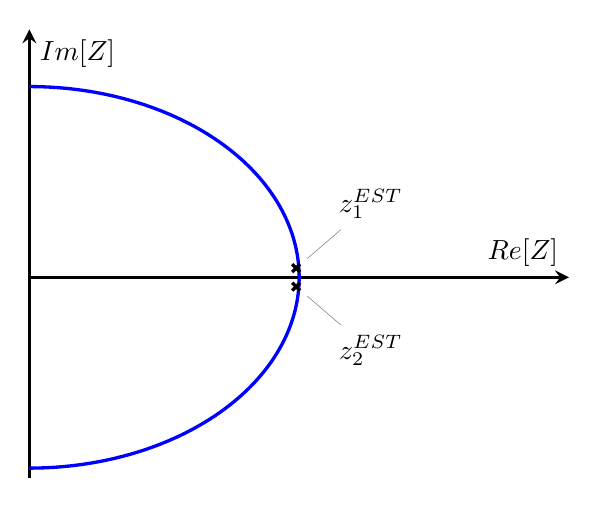
\begin{tikzpicture} 
\begin{axis}[very thick,
                     samples = 100,
                     ytick={-10,10},
                     xlabel = {$Re[Z]$},
                     ylabel = {$Im[Z]$},
                     xmin = 0,
                     xmax = 2,
                     ymin = -1.05,
                     ymax = 1.3,
                     axis x line = middle,
                     axis y line = middle,
                     ticks = none]
            \addplot [domain=-180:180, samples=1000, color=blue] ({cos(x)},{sin(x)});
            \addplot[mark=x] coordinates {(0.988862,0.0484835)} node[pin=50:{$z_{1}^{EST}$}]{};
            \addplot[mark=x] coordinates {(0.988862,-0.0484835)} node[pin=-50:{$z_{2}^{EST}$}]{};
        \end{axis}
        
\end{tikzpicture}
\end{center}
\caption{Círculo unitário para o sistema estável.}
\label{graph:1} 
\end{figure}


\begin{figure}[H]
\begin{center}
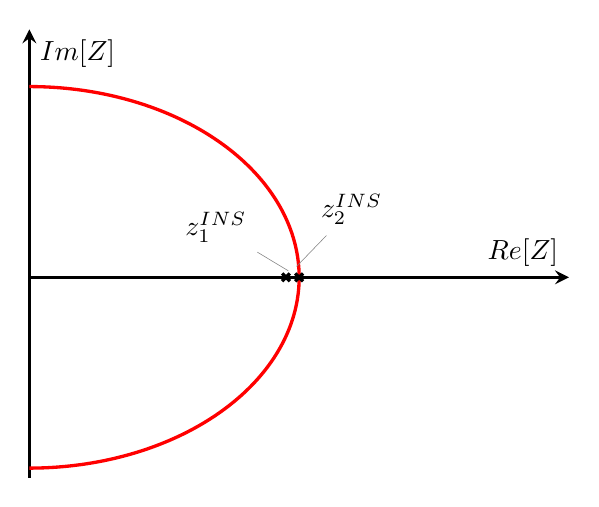
\begin{tikzpicture} 
\begin{axis}[very thick,
                     samples = 100,
                     ytick={-10,10},
                     xlabel = {$Re[Z]$},
                     ylabel = {$Im[Z]$},
                     xmin = 0,
                     xmax = 2,
                     ymin = -1.05,
                     ymax = 1.3,
                     axis x line = middle,
                     axis y line = middle,
                     ticks = none]
            \addplot [domain=-180:180, samples=1000, color=red] ({cos(x)},{sin(x)});
            \addplot[mark=x] coordinates {(1,0)} node[pin=150:{$z_{1}^{INS}$}]{};
            \addplot[mark=x] coordinates {(0.951229,0)} node[pin=60:{$z_{2}^{INS}$}]{};
        \end{axis}
        
\end{tikzpicture}
\end{center}
\caption{Círculo unitário para o sistema instável.}
\label{graph:2} 
\end{figure}


Pela posição dos polos do sistema estável estar distante da origem, justifica-se o fato de sua resposta levar um tempo maior para se estabilizar ($T_S \approx 4s$)

\subsubsection{Estabilidade assintótica}

De acordo com o teorema da estabilidade assintótica, com a ausência de cancelamento de polos e zeros, um sistema digital LT é dito estável se os seus polos pertencem ao círculo unitário aberto e marginalmente estável se seus polos pertencem ao círculo unitário fechado e sem polos repetidos no círculo.

Dessa forma, considerando os polos dos sistemas em malha aberta apresentados nas equações \ref{polo:z:est}, \ref{polo:z:ins:1} e \ref{polo:z:ins:2},  o sistema proposto como estável, do ponto de vista da estabilidade assintótica, de fato é estável, pois todos os seus polos pertencem ao círculo unitário aberto. Enquanto que o sistema considerado estável, do ponto de vista da estabilidade assintótica ele é marginalmente estável, pois um dos polos habita a periferia do círculo unitário fechado.

\subsubsection{Estabilidade BIBO}

A estabilidade Bounded Input and Bounded Output (BIBO) prevê que se uma entrada limitada inserida no sistema e este responder com uma saída limitada, assim o teorema da estabilidade BIBO propõe para que um sistema seja BIBO estável, sua resposta ao impulso seja totalmente somável. Do ponto de vista dos polos da função de transferência, o sistema discreto no tempo e linear só será estável se seus polos habitarem o interior do círculo unitário.

Portanto, considerando os polos dos sistemas em malha aberta, o sistema estável também é BIBO estável, enquanto que o sistema instável é considerado BIBO instável, pois este possui um polo que habita a periferia do círculo unitário. 

\subsubsection{Critério de Routh-Hurwitz}

Para aplicar o critério de estabilidade de Routh-Hurwitz há a necessidade de realizar a transformação bilinear dada pela equação abaixo, de forma a mapear a função de transferência do plano z para o plano s, de forma a avaliar o critério de acordo com o que se realizava para sistemas analógicos, ao verificar a mudança dos sinais dos elementos da tabela:

\begin{center}
    $z = \frac{1+s}{1-s}$
\end{center}

Assim, ao aplicar a transformação bilinear na função de transferência padrão da equação \ref{z:default}, obtém-se a forma:

\begin{center}
    $H(s) = \frac{(d-c)s^2 - (2d)s + (d+c)}{(1+a+b)s^2 (2-2b)s + (1-a+b)}$
\end{center}

De forma que a tabela de Routh padrão, já considerando os elementos a serem calculados, será:

\begin{table}[h]
\centering
%\caption{Tabela. }\label{table:rotuh}
\begin{tabular}{l|ccc}
 $s^2$ & $1+a+b$ & $1-a+b$ & 0 \\ \hline
 $s^1$ & $2-2b$ & 0 & 0 \\ \hline
 $s^0$ & $-\frac{det\left(\begin{bmatrix} 1+a+b & 1-a+b \\ 2-2b & 0 \end{bmatrix}\right)}{2-2b}$ & 0 & 0 \\ \hline
\end{tabular}
\end{table}

Aplicando os devidos coeficientes das funções de transferência do sistema considerado estável e o instável, tem-se as funções de transferência transformadas da equação \ref{routh:est} para o sistema considerado estável e a equação \ref{routh:ins} para o sistema considerado instável.

\begin{equation} \label{routh:est}
    H(s) = \frac{-3.3e-6 s^2 - 9.866e-4 s + 9.899e-4}{3.9579227s^2 + 0.0396026s + 0.0024747}
\end{equation}

\begin{equation} \label{routh:ins}
    H(s) = \frac{-1.581e-4s^2 - 0.0193546s + 0.0195127}{3.9024588s^2 + 0.0975412s}
\end{equation}

Assim, as tabelas de Routh para cada uma das situações será dada em seguida.

Para a tabela \ref{table:routh:est}, observa-se que o sistema que antes foi considerado estável, de fato é estável com todos os polos no semiplanos esquerdo, pois a primeira coluna da tabela de Routh não possui troca de sinais.

\begin{table}[h]
\centering
\caption{Tabela de Routh para o sistema considerado estável.}\label{table:routh:est}
\begin{tabular}{l|ccc}
 $s^2$ & 3.9579227 & 0.0024747 & 0 \\ \hline
 $s^1$ & 0.0396026 & 0 & 0 \\ \hline
 $s^0$ & 0.0024747 & 0 & 0 \\ \hline
\end{tabular}
\end{table}

Para o sistema considerado instável, a linha correspondente a $s^0$ será composta por zeros, dessa forma recorre-se ao polinômio da linha anterior e os coeficientes da derivada desse polinômio irão compor os coeficientes da linha que antes era nula, de forma que:

\begin{center}
    $P(s) = 0.0975412s^1$\vspace{4pt}\\
    $\frac{dP(s)}{ds} = 0.0975412s^0$
\end{center}

Essa linha inteira de zeros aparece quando existe um polinômio estritamente par ou estritamente ímpar que for um fator do polinômio original. Porém, ao observar a tabela \ref{routh:ins}, não há mudança de sinal nas duas últimas linhas, indicando que não há polos no semiplano direito. Como o polinômio é considerado par e não possui polos no semiplano da direita, também não o possui no semiplano da esquerda, indicando que este último polo se encontra na origem. Dessa forma, como não há mudança de sinal da primeira para a segunda linha, há um polo no semiplano esquerdo e, devido a conclusão anterior, há um polinômio na origem, deixando o sistema de fato instável.

\begin{table}[h]
\centering
\caption{Tabela de Routh para o sistema considerado instável.}\label{table:routh:ins}
\begin{tabular}{l|ccc}
 $s^2$ & 3.9024588 & 0 & 0 \\ \hline
 $s^1$ & 0.0975412 & 0 & 0 \\ \hline
 $s^0$ & 0.0975412 & 0 & 0 \\ \hline
\end{tabular}
\end{table}

A existência do polo na origem poderia ser interpretado pelo próprio polinômio do denominador, mas como estava sendo realizada a análise por Routh-Hurwitz, decidiu-se completá-la. O polo na origem também poderia ser identificado a partir do polinômio da linha $s^1$, pois uma vez que este é de grau 1, ele não poderia ter raízes pares.

\subsection{Representação dos sistemas}

\subsubsection{Espaço de estados}

Para o sistema estável, considerando as matrizes encontradas nas equações \ref{est:6}, \ref{est:7} e para C e D em \ref{est:5} e atribuindo $h = 0.01 s$ para o período de amostragem, tem-se que a representação em espaço de estados discreto para esse sistema será:

\begin{equation} \label{ss:est}
\centering
\left \{
\begin{array}{cc}
x[n+1] = \begin{bmatrix} 0.9987586 & 0.0098965 \\ -0.2474135 & 0.9789655 \end{bmatrix} x[n] + \begin{bmatrix} 0.0004966 \\ 0.0989654 \end{bmatrix} u[n] \\
y[n] = \begin{bmatrix} 1 & 0  \end{bmatrix} x[n] \\
\end{array}
\right.
\end{equation}


Para o sistema instável, considerando as matrizes encontradas nas equações \ref{ins:5}, \ref{ins:6} e para C e D em \ref{ins:4} e atribuindo $h = 0.1 s$ para o período de amostragem, tem-se que a representação em espaço de estados discreto para esse sistema será:

\begin{equation} \label{ss:ins}
\centering
\left \{
\begin{array}{cc}
x[n+1] = \begin{bmatrix} 1 & 0.0975412 \\ 0 & 0.9512294 \end{bmatrix} x[n] + \begin{bmatrix} 0.0098354 \\ 0.1950823 \end{bmatrix} u[n] \\
y[n] = \begin{bmatrix} 1 & 0  \end{bmatrix} x[n] \\
\end{array}
\right.
\end{equation}


\subsubsection{Resposta em frequência}

Considerando as plantas estudadas neste trabalho no formato da função de transferência discreta da equação \ref{z:default}, sua equação diferença será na forma da equação \ref{eqdif:default}.

\begin{equation} \label{eqdif:default}
    y[n+2]-ay[n+1]+by[n]=cu[n+1]+du[n]
\end{equation}

Dessa forma, considerando que $y[n] = Be^{j\omega n}$ e $u[n] = Ae^{j\omega n}$ e substituindo na equação diferença, tem-se que a resposta do sistema pode ser expressa como:

\begin{center}
    $Be^{j \omega (n+2)} - aBe^{j \omega (n+1)} + bBe^{j \omega n} = cAe^{j \omega (n+1)} + dAe^{j \omega n} $\vspace{4pt}\\
    $Be^{j \omega n} (e^{j \omega 2} - ae^{j \omega } + b) = Ae^{j \omega n} (ce^{j \omega } + d)$ \vspace{4pt}\\
    $B = A \frac{ce^{j \omega}+d}{e^{j 2\omega} - ae^{j \omega} + b} = A H(e^{j \omega})$ \vspace{4pt}\\
\end{center}
\begin{equation} \label{freqrep:y}
    y[n] = H(e^{j \omega}) Ae^{j \omega n}
\end{equation}

Em que a função de transferência na representação em resposta de frequência é dada na forma da equação \ref{freqrep:ft}.

\begin{equation} \label{freqrep:ft}
    H(e^{j \omega}) = \frac{ce^{j \omega}+d}{e^{j 2\omega} - ae^{j \omega} + b}
\end{equation}

Dessa forma, a função de transferência discreta na forma da resposta em frequência para a planta estável e instável podem ser observadas na equações \ref{freqrep:est} e \ref{freqrep:ins}, respectivamente, ao substituir os devidos coeficientes.

\begin{equation} \label{freqrep:est}
    H_{est}(e^{j \omega}) = \frac{0.0004966e^{j \omega}+0.0004933}{e^{j 2\omega} - 1.977724e^{j \omega} + 0.9801987}
\end{equation}

As curvas de módulo e fase estão apresentadas na figura \ref{freq:est}, para a planta estável e na figura \ref{freq:ins}, para a planta instável. Observa-se, além da periodicidade da resposta, que as curvas de fase são semelhantes. A curva de módulo para a planta estável possui ganhos baixos, na faixa abaixo de 0dB. A planta instável possui ganhos maiores, inclusive um ganho que tende ao infinito em nível DC (foi omitido para não distorcer o gráfico, pois é da ordem de 284 dB), justificando o fato de que a entrada do tipo degrau a instabilizou, enquanto que a senoide que possui componentes frequenciais mais elevadas, não o fez.

\begin{figure}[H]
\begin{center}
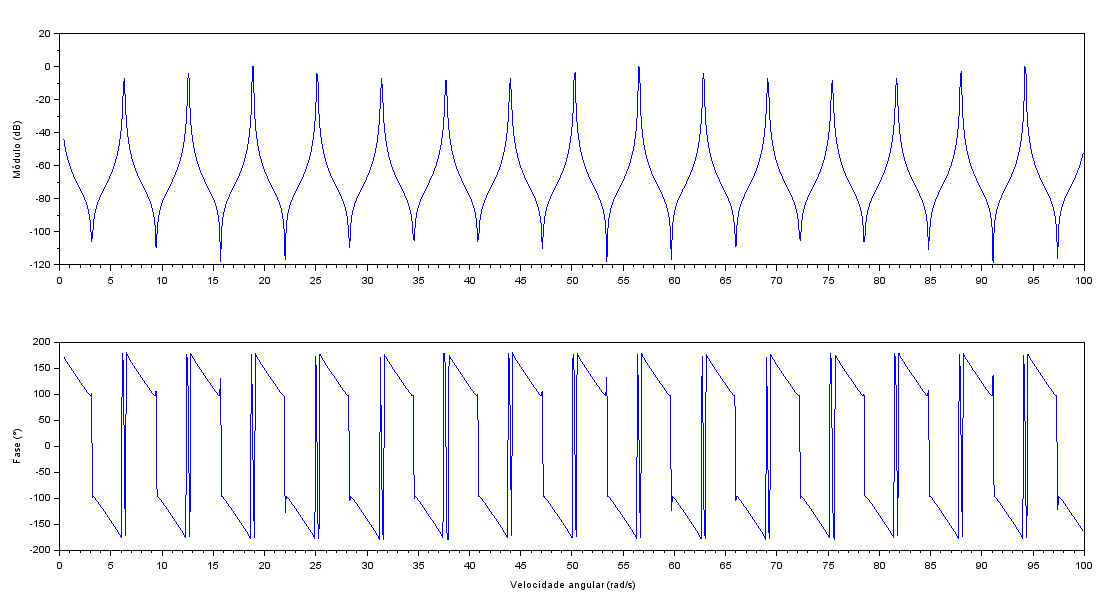
\includegraphics[width=15cm]{images/freq/estavel_freq.png}
\caption{Curvas de módulo e frequência para a planta estável.}
\label{freq:est} 
\end{center}
\end{figure}

\begin{equation} \label{freqrep:ins}
    H_{ins}(e^{j \omega}) = \frac{0.0098354e^{j \omega}+0.00967728}{e^{j 2\omega} - 1.9512294e^{j \omega} + 0.9512294}
\end{equation}



\begin{figure}[H]
\begin{center}
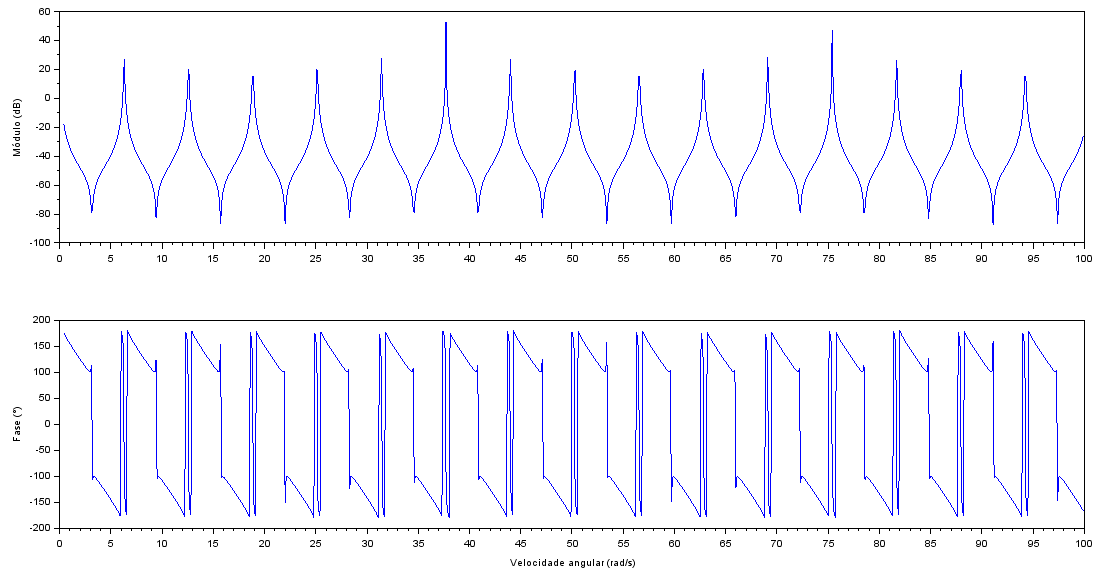
\includegraphics[width=15cm]{images/freq/instavel_freq.png}
\caption{Curvas de módulo e frequência para a planta instável.}
\label{freq:ins} 
\end{center}
\end{figure}

\subsection{Lugar das raízes}

Para entender o comportamento dos polos do sistema discreto em malha fechada é necessário avaliar o diagrama do lugar das raízes de ambos os sistemas. Dessa forma foi utilizado o software computacional MATLAB para auxiliar na construção do lugar das raízes.

Para o sistema instável, observa-se no diagrama que ambos os polos se encontram no eixo real no polo de 0.975 e deixam o eixo, iniciando a ter uma resposta oscilatória para poucos valores de ganho. Em seguida os polos deixam o círculo de raio unitário, garantindo que a resposta seja sempre instável. Eles voltam a se encontrar no eixo real por volta de -2.94, mas ainda instável. Para valores maiores de ganho, um polo retorna à periferia do círculo unitário e o outro tende ao infinito. Para a planta estável o comportamento é igual, com a exceção de que os polos não se encontram no eixo real, pois já partem para a instabilidade a partir de polos complexos.

\begin{figure}[H]
\begin{center}
    \subfigure{             
        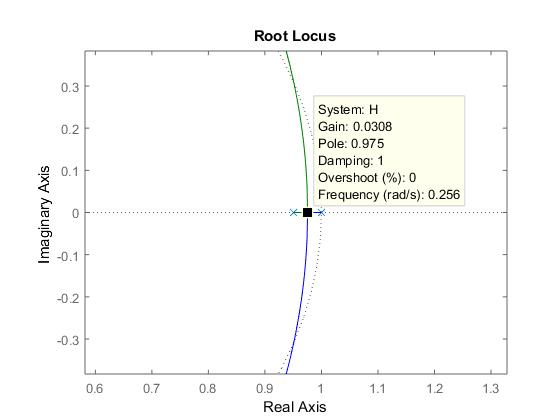
\includegraphics[width=7.5cm]{images/RL/RL_ins_1.jpg}  
        \label{rl:ins:1}
    }
    \subfigure{                                              
        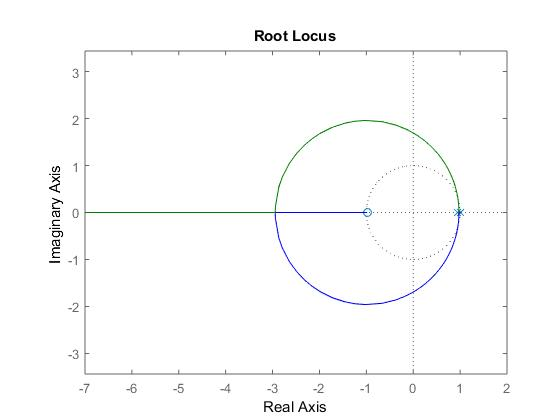
\includegraphics[width=7.5cm]{images/RL/RL_ins_2.jpg}
        \label{rl:ins:1}
    }                
\end{center}
\caption{Lugar das raízes para a planta instável em malha aberta.}
\label{rl:ins} 
\end{figure}

\begin{figure}[H]
\begin{center}
    \subfigure{             
        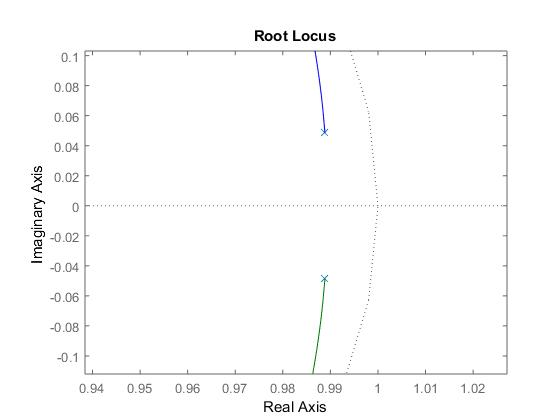
\includegraphics[width=7.5cm]{images/RL/RL_est_1.jpg}  
        \label{rl:est:1}
    }
    \subfigure{                                              
        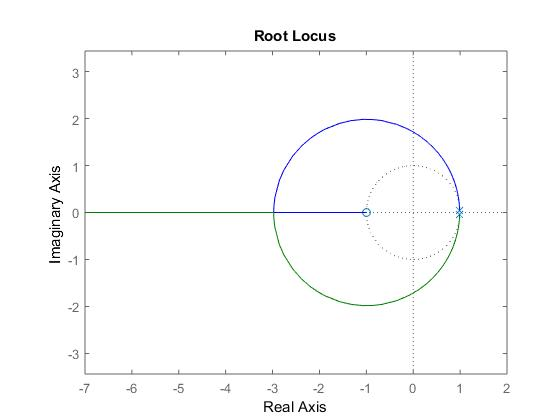
\includegraphics[width=7.5cm]{images/RL/RL_est_2.jpg}
        \label{rl:est:1}
    }                
\end{center}
\caption{Lugar das raízes para a planta instável em malha aberta.}
\label{rl:est} 
\end{figure}


\subsection{Controladores}

Esta seção será responsável pelo detalhamento do projeto dos controladores para a planta estável e instável. Uma vez que o projeto é livre, será escolhido o método de projeto pelo lugar das raízes para ambas as plantas analógicas, sendo necessário discretizar o controlador, a posteriori. 

O sistema em malha fechada com controlador deve possuir erro de regime permanente nulo para uma entrada do tipo degrau, tempo de estabilização menor ou igual que meio segundo ($T_S \leq 0.5s$) e percentual de ultrapassagem menor ou igual a $5\%$ ($OS(\%) \leq 5\%$). De acordo com os dados da tabela \ref{table:2} - que apesar de se referirem aos sistemas discretos, também são iguais para a versão analógica - observa-se que ambos os sistemas não cumprem os requisitos, exceto o requisito de erro nulo ao degrau que a planta instável já cumpre, pois possui um integrador. 

Dessa forma, espera-se que o modelo das plantas sigam: PID para o sistema estável, pois necessita de melhor desempenho e erro de regime nulo; PD para o sistema instável para melhorar apenas o desempenho.

De acordo com os requisitos de desempenhos que devem ser impostos, os elementos da equação \ref{tran:1} podem ser relacionados com os requisitos de desempenho de acordo com o proposto em OGATA (2009) e com a equação \ref{polinom:3} para o coeficiente de amortecimento e percentual de ultrapassagem e a equação \ref{polinom:4} para a frequência natural e o tempo de estabilização. Os requisitos de desempenho utilizados obedecerão o valor limítrofe. 

\begin{equation} \label{polinom:3}
    \xi = \frac{-ln(OS)}{\sqrt{\pi^2+ln^2(OS)}} = 0.6901 \approx 0.7
\end{equation}
\begin{equation} \label{polinom:4}
    \omega_n = \frac{4}{T_S\xi} = 11.428 rad/s
\end{equation}

A partir do polinômio arbitrário observa-se que as raízes pretendidas e que estabelecem os critérios de desempenho são: $s_{1,2} = -8 \pm j8.16122$. Assim, o projeto pelo lugar das raízes vai garantir que estes polos sejam alcançados.

O PID desejado será na forma:
\begin{equation} \label{pid:0}
    C(s) = \frac{k_c\tau_d\left(s+\frac{1}{2\tau_d}\right)^2}{s}
\end{equation}

Vale destacar que o PID está na forma simplificada, considerando o termo integrativo quatro vezes o derivativo, restando apenas o derivativo com dois polos iguais.

Enquanto que o PD será:
\begin{equation} \label{pid:1}
    C(s) = k_c\tau_d\left(s+ \frac{1}{\tau_d}\right)
\end{equation}

Para encontrar os controlador PID discreto, será utilizada a transformação bilinear:

\begin{center}
    $s = \frac{1}{h}ln(z) \approx \frac{2}{h}\left[\frac{z-1}{z+1}\right]$\vspace{4pt}\\
\end{center}

FADALI (2013) resume o controlador PID, discretizado de acordo com a transformação linear na equação \ref{trans:bi:2}. Vale destacar que a transformação do controlador PID resulta em um PD digital. Assim, sendo $c=\frac{2}{h}$, tem-se:

\begin{comment}
O controlador possui um zero para melhorar o transitório e um polo em $z=-1$. O polo em $z=-1$ corresponde a uma resposta em frequência não limitada e deve ser eliminado. Mas se eliminá-lo, o controlador será irrealizável. Assim, uma aproximação é trocar o polo por outro na origem, resultando no controlador PD analógico transformado, pois este está associado a uma resposta mais rápida que decai rapidamente, e possui distorção. Essa variação resulta em uma distorção adicional ao filtro analógico e dobra ao ganho DC, sendo necessário reduzir $K$ pela metade, além do ajuste de ganho.
\end{comment}


\begin{center}
   $C(z) = K\frac{(s+a)(s+b)}{s}\Big|_{s=c\left[\frac{z-1}{z+1}\right]} = K\frac{(a+c)(b+c)}{c}\frac{\left[z+\left(\frac{a-c}{a+c}\right)\right]\left[z+\left(\frac{b-c}{b+c}\right)\right]}{(z+1)(z-1)}$
\end{center}

\begin{equation} \label{trans:bi:2}
    C(z) = \frac{K}{2}\frac{(a+c)(b+c)}{c}\frac{\left[z+\left(\frac{a-c}{a+c}\right)\right]\left[z+\left(\frac{b-c}{b+c}\right)\right]}{z(z-1)}
\end{equation}

O controlador possui um zero para melhorar o transitório e um polo em $z=-1$. O polo em $z=-1$ corresponde a uma resposta em frequência não limitada e deve ser eliminado. Mas se eliminá-lo, o controlador será irrealizável. Assim, uma aproximação é trocar o polo por outro na origem associado a uma resposta rápida e com distorções que podem ser resolvidas cortando o ganho DC pela metade e demais ajustes. O polo em $z=1$ introduzido pelo PID discreto contribui para anular o erro em regime permanente. 

Para o controlador PD será utilizada a aproximação da derivada para frente (por não introduzir polo no controlador, como a aproximação para trás faz, podendo gerar distorções):

\begin{equation} \label{trans:bi:1}
    s \rightarrow \frac{z-1}{h}
\end{equation}

\subsubsection{Sistema estável}

Para realizar a análise a partir do lugar das raízes, vale lembrar que existem um par de polos devido à planta ($P1$ e $P2$), dois zeros iguais ($Z$) e um polo na origem ($P3$) devidos ao PID. Assim, as condições para que um dos polos de $s_{1,2}=s_i$ pertençam ao lugar das raízes, deve seguir o critério de fase e módulo.

O critério de fase permite encontrar o ângulo relativo dos zeros com o polo de referência. Os demais ângulos são facilmente encontrados a partir de relações trigonométricas ($\theta_{P1} = 155.0123^{\circ}$, $\theta_{P2} = 118.19^{\circ}$ e $\theta_{P3} = 134.43^{\circ}$).

\begin{equation} \label{pid:2}
    \angle A(s_i) = 2 \theta_Z - \theta_{P1} - \theta_{P2} - \theta_{P3} = 180^{\circ} => \theta_Z = 112.816^{\circ}
\end{equation}

O termo derivativo pode ser facilmente encontrado por relações trigonométricas, como: $\tau_d = 0.11369$.

A condição de módulo permite encontrar o ganho proporcional, uma vez que o termo derivativo fora encontrado. Ela deve ser computada a partir da distância relativa de todos os polos e zeros ao polo de referência. As relações são facilmente encontradas a partir de relações trigonométricas ($A_Z = 79.58$, $A_{P1} = 7.72$, $A_{P2} = 14.81$ e $A_{P3} = 11.42$).

\begin{equation} \label{pid:4}
    |A(s_i)| = \frac{k_c \tau_d A_Z^2}{A_{P1} A_{P2} A_{P3}} = 1 => k_c = 144.54
\end{equation}

Assim, a forma final do controlador analógico será:

\begin{equation} \label{pid:5}
    C(s) = 16.4327s+144.5387+\frac{317.83}{s}
\end{equation}

Ao realizar a transformação bilinear por meio da equação \ref{trans:bi:2}, obtém-se o controlador discreto.

\begin{equation} \label{trans:bi:3}
    C(z) = 1716.3343\frac{z^2-1.9139z+0.9157}{z(z-1)}
\end{equation}

Ao simular o sistema discreto em malha fechada e com o controlador para uma entrada do tipo degrau e compará-lo com a mesma situação para o sistema em tempo contínuo, obtém-se a figura \ref{mf:1}.


\begin{figure}[H]
\begin{center}
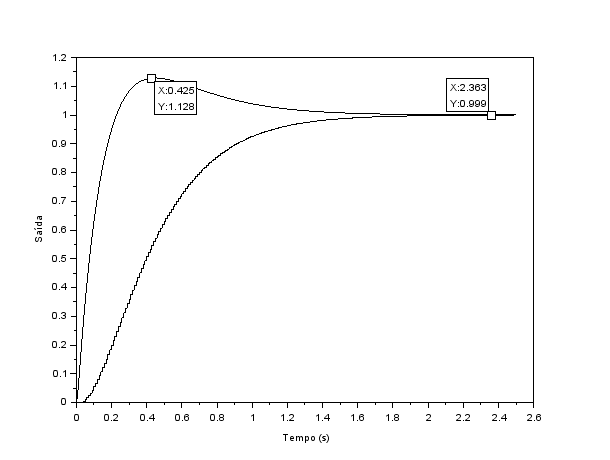
\includegraphics[width=12cm]{images/mf/mf_estavel.png}
\caption{Comparação entre a saída em tempo contínuo e tempo discreto para o sistema estável em malha fechada e com controlador.}
\label{mf:1} 
\end{center}
\end{figure}

A partir da análise da figura, observa-se que a resposta para o sistema contínuo possuiu uma ultrapassagem maior que a esperada pelo projeto do controlador, ou seja, ao invés de  5\% obteve-se cerca de 12\%, mas o tempo de estabilização se manteve em cerca de 0.5s. Porém, em termos da resposta discreta, a transformação bilinear causou distorções a ponto de contribuir para a redução do percentual de ultrapassagem (anulando-o), mas com o prejuízo de dobrar o tempo de estabilização (1s). Ambas alcançaram o regime permanente de acordo com a referência degrau. Essa compensação de desempenhos entre as representações foi devido ao fator de ganho do controlador ser ajustado para a metade, devido às distorções geradas pelo polo na origem do controlador discreto. Em conclusão, os valores são bastante aceitáveis, uma vez que o critério de tempo de estabilização de 0.5s foi decidido com base em eventuais distorções.

Por fim, ao inserir o controlador, o lugar das raízes para o sistema em malha fechada foi amplamente alterado, com os polos mantendo-se sempre dentro do círculo unitário e com polos que para um ganho infinito tendem a -0.993 e 0.957. Enquanto que este último é um polo duplo devido a inserção do polo em z=1 do controlador (polo na origem do plano s).

\begin{figure}[H]
\begin{center}
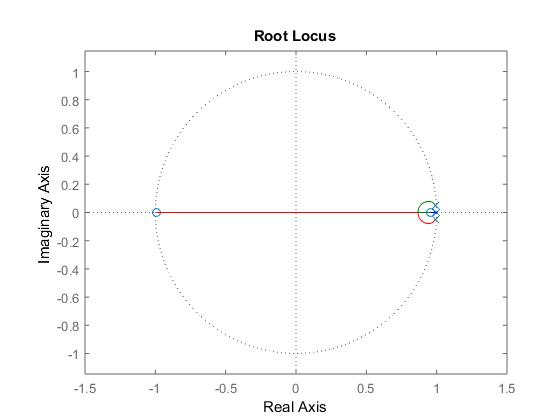
\includegraphics[width=12cm]{images/RL/RL_est_C.jpg}
\caption{Lugar das raízes para a planta estável com o controlador.}
\label{rl:ins:c} 
\end{center}
\end{figure}

\subsubsection{Sistema instável}

Para realizar a análise a partir do lugar das raízes, vale lembrar que a planta possui um polo na origem ($P2$) e outro no eixo real ($P1$). A planta irá inserir apenas um zero ($Z$).

Analogamente ao projeto anterior, os ângulos podem ser encontrados por relações trigonométricas ($\theta_{P1} = 132.582^{\circ}$ e $\theta_{P2} = 134.53^{\circ}$) e o ângulo do zero será encontrado pelo critério de fase.

\begin{equation} \label{pid:6}
    \angle A(s_i) = \theta_Z - \theta_{P1} - \theta_{P2} = 180^{\circ} => \theta_Z = 87.112^{\circ}
\end{equation}

O termo derivativo pode ser facilmente encontrado por relações trigonométricas, como: $\tau_d = 0.11888$.

Os módulos relativos ao polo desejado são facilmente encontrados a partir de relações trigonométricas para garantir a condição de módulo ($A_Z = 8.1716$, $A_{P1} = 11.084$ e $A_{P2} = 11.4282$).

\begin{equation} \label{pid:7}
    |A(s_i)| = \frac{k_c \tau_d A_Z}{A_{P1} A_{P2} } = 1 => k_c = 130.395
\end{equation}

Assim, a forma final do controlador analógico será:

\begin{equation} \label{pid:8}
    C(s) = 15.5014s + 130.395
\end{equation}

Ao realizar a transformação por meio da aproximação da derivada para a frente por meio da relação \ref{trans:bi:1}, obtém-se o controlador discreto.

\begin{equation} \label{trans:bi:4}
    C(z) = 155.014(z-0.15882)
\end{equation}

Ao simular o sistema discreto em malha fechada e com o controlador para uma entrada do tipo degrau e compará-lo com a mesma situação para o sistema em tempo contínuo, obtém-se a figura \ref{mf:2}.

\begin{figure}[H]
\begin{center}
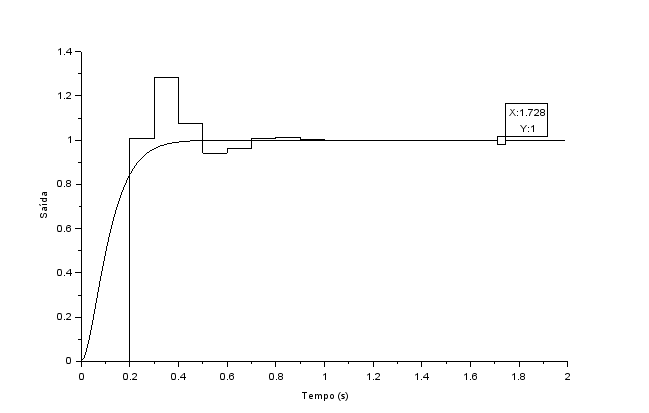
\includegraphics[width=12cm]{images/mf/mf_instavel.png}
\caption{Comparação entre a saída em tempo contínuo e tempo discreto para o sistema instável em malha fechada e com controlador.}
\label{mf:2} 
\end{center}
\end{figure}

A partir da análise da figura, observa-se que a relação de troca que antes houve para o sistema estável, não aconteceu aqui. No sistema contínuo, apesar de ter sido projetado o percentual de ultrapassagem de 5\%, na simulação ele anulou a ultrapassagem, possuindo uma resposta bem suave e que alcança a referência degrau. 

Enquanto isso, o sistema discretizado cumpriu o requisito de tempo e estabilização (0.5s), alcançando em 5 amostras (tempo de amostragem de 0.1s), mas o percentual de ultrapassagem foi deveras alto, cerca de 28\% (sinal máximo de 1.28). Essa distorção pode ser considerada devido a aproximação adotada (derivada para frente) e diretamente ligado ao tempo de amostragem baixo. Isso se justifica, pois em experimentos, ao reduzir o período de amostragem ($/10$) a resposta suavizou e se aproximou da resposta contínua. 

Outra opção mais fácil de implementar foi dobrar o ganho derivativo ou reduzir o ganho proporcional do controlador. As saídas para ambas as opções apresentam sobrepostas na figura \ref{mf:3}, não sendo necessário identificar uma ou outra, pois possuem comportamento bem semelhante: percentual de ultrapassagem nulo e tempo de estabilização de 0.6s (6 amostras).

\begin{figure}[H]
\begin{center}
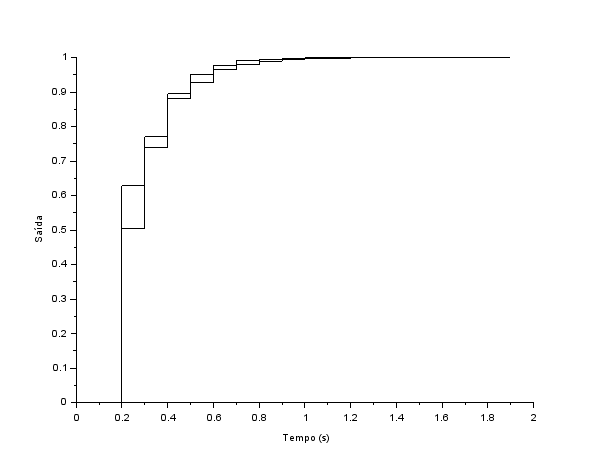
\includegraphics[width=12cm]{images/mf/sobreposto.png}
\caption{Comparação entre a saída discreta com controlador ajustado.}
\label{mf:3} 
\end{center}
\end{figure}

Por fim, ao inserir o controlador, o lugar das raízes para o sistema em malha fechada foi amplamente alterado, com os polos mantendo-se sempre dentro do círculo unitário e com polos que para um ganho infinito tendem a -0.984 e 0.579.

\begin{figure}[H]
\begin{center}
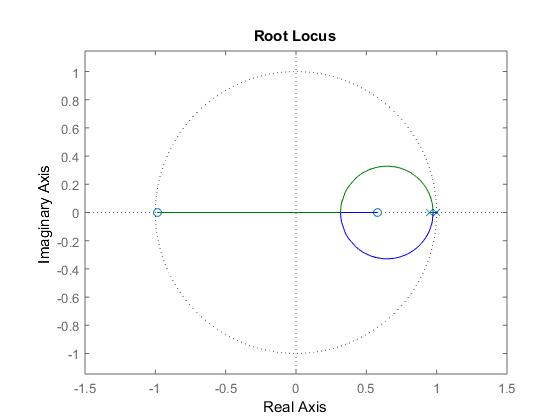
\includegraphics[width=12cm]{images/RL/RL_ins_C.jpg}
\caption{Lugar das raízes para a planta instável com o controlador.}
\label{rl:ins:c} 
\end{center}
\end{figure}

\subsection{Comparação com o controlador \textit{dead beat}}

No projeto do \textit{dead beat} foi considerada a forma padrão (equação \ref{z:default}) das plantas discretas trabalhadas. Como o denominador e o numerador da planta tornam-se o numerador e denominador do controlador, respectivamente, e com uma quantidade $n$ de polos em $z=1$ adicionados no controlador para garantir a resposta desejada. Como a diferença no grau do denominador para o numerador da planta difere de 1, implica que $n=1$. Assim, o formato dos \textit{dead beats} utilizados neste trabalho seguema forma:

\begin{center}
    $C(z) = \frac{z^2-az+b}{(cz+d)(z-1)}$
\end{center}

Com o controlador pronto e aplicado ao sistema realimentado negativamente, assim como nos sistemas anteriores com seus respectivos controladores. Na intenção de comparar os controladores trabalhados em tópicos anteriores com o \textit{dead beat}, não adianta recorrer à saída, pois ao considerar o sistema com o \textit{dead beat}, esta será apenas a entrada global do sistema com uma quantidade $n$ de atrasos. Assim, basta recorrer ao sinal de controle, pois este indica o quão rígido o controle foi. Devido à natureza do \textit{dead beat}, espera-se que os sinais de controle por ele gerados possua amplitudes maiores e banda de frequência mais ampla, enquanto que o controlador tradicional possui uma saída mais suave.

Sendo a linguagem dos fatos a mais eloquente, permite-se passar diretamente para os dados experimentais, frutos da simulação, que autorizam discutir a respeito da hipótese proferida.


\begin{figure}[H]
\begin{center}
    \subfigure[\textit{Dead beat}]{             
        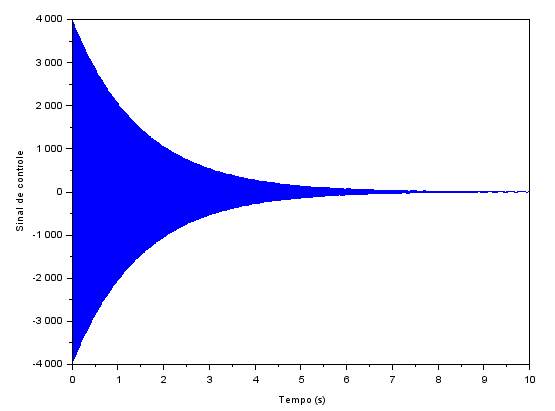
\includegraphics[width=7.5cm]{images/deadbeat/deadbeat_est_sincont.png}  
        \label{deadbeat:est:1}
    }
    \subfigure[PID]{                                              
        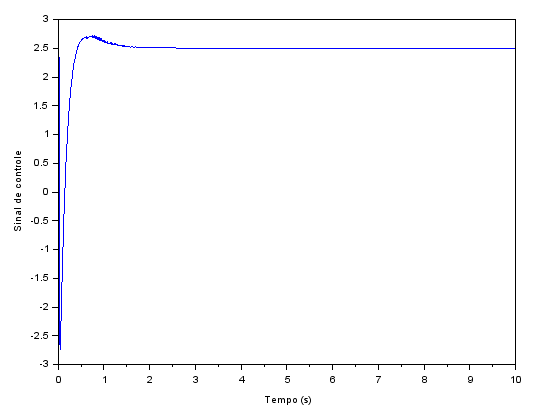
\includegraphics[width=7.5cm]{images/deadbeat/controller_est_sincont.png}
        \label{deadbeat:est:2}
    }                
\end{center}
\caption{Comparação entre os sinais de controle gerados pelos controladores (a) \textit{dead beat} e o (b) PID para a planta estável e com a entrada do tipo degrau.}
\label{deadbeat:est} 
\end{figure}

\begin{figure}[H]
\begin{center}
    \subfigure[\textit{Dead beat}]{             
        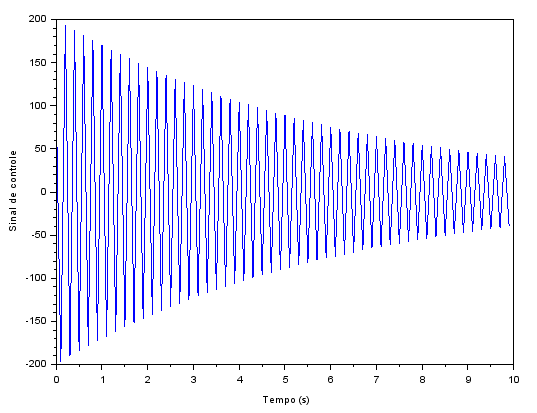
\includegraphics[width=7.5cm]{images/deadbeat/deadbeat_ins_sincont.png}  
        \label{deadbeat:ins:1}
    }
    \subfigure[PD]{                                              
        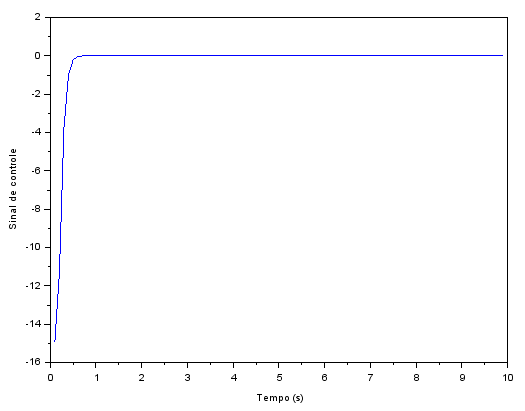
\includegraphics[width=7.5cm]{images/deadbeat/controller_ins_sincont.png}
        \label{deadbeat:ins:2}
    }                
\end{center}
\caption{Comparação entre os sinais de controle gerados pelos controladores (a) \textit{dead beat} e o (b) PD para a planta instável e com a entrada do tipo degrau.}
\label{deadbeat:ins} 
\end{figure}

De acordo com as imagens \ref{deadbeat:est} e \ref{deadbeat:ins}, observa-se que a excursão da amplitude dos sinais de controle pelos \textit{dead beats} foi muito mais elevada que para os outros controladores: PID e PD. Ao longo do tempo o sinal tende a estabilizar. A frequência também se mostra elevada, enquanto que para os controladores tradicionais, as respostas são bem suaves e que tendem a seguir o formato da saída do sistema. 

Um fato importante, e que foi omitido no gráfico para evitar distorções, é que os controladores PID e PD possuem, em suas primeiras amostras, uma grande amplitude do sinal de controle. Isto é devido às parcelas derivativas do controlador que deriva a entrada degrau, resultando em uma taxa de crescimento infinita. Porém, com o tempo, esses valores são corrigidos por meio do próprio controle para valores relativos à dinâmica do sistema.



\pagebreak